\documentclass[12pt]{article}
\usepackage[left=1cm, right=1cm, top=2cm,bottom=1.5cm]{geometry} 

\usepackage[parfill]{parskip}
\usepackage[utf8]{inputenc}
\usepackage[T2A]{fontenc}
\usepackage[russian]{babel}
\usepackage{enumitem}
\usepackage[normalem]{ulem}
\usepackage{amsfonts, amsmath, amsthm, amssymb, mathtools}

\usepackage{fancyhdr}
\pagestyle{fancy}
\renewcommand{\headrulewidth}{1.5pt}
\renewcommand{\footrulewidth}{1pt}

\usepackage{graphicx}
\usepackage[figurename=Рис.]{caption}
\usepackage{subcaption}
\usepackage{float}

%%Наименование папки откуда забирать изображения
\graphicspath{ {./images/} }

%%Изменение формата для ввода доказательства
\renewcommand{\proofname}{$\square$  \nopunct}
\renewcommand\qedsymbol{$\blacksquare$}

\addto\captionsrussian{%
	\renewcommand{\proofname}{$\square$ \nopunct}%
}
%% Римские цифры
\newcommand{\RN}[1]{%
	\textup{\uppercase\expandafter{\romannumeral#1}}%
}

%% Для удобства записи
\newcommand{\MR}{\mathbb{R}}
\newcommand{\MQ}{\mathbb{Q}}
\newcommand{\MI}{\mathrm{I}}
\newcommand{\MJ}{\mathrm{J}}
\newcommand{\MH}{\mathrm{H}}
\newcommand{\MT}{\mathrm{T}}
\newcommand{\MU}{\mathcal{U}}
\newcommand{\MV}{\mathcal{V}}
\newcommand{\VN}{\varnothing}
\newcommand{\VE}{\varepsilon}

\theoremstyle{definition}
\newtheorem{defn}{Опр:}
\newtheorem{rem}{Rm:}
\newtheorem{prop}{Утв.}
\newtheorem{exrc}{Упр.}
\newtheorem{lemma}{Лемма}
\newtheorem{theorem}{Теорема}
\newtheorem{corollary}{Следствие}

\newenvironment{cusdefn}[1]
{\renewcommand\thedefn{#1}\defn}
{\enddefn}

\DeclareRobustCommand{\divby}{%
	\mathrel{\text{\vbox{\baselineskip.65ex\lineskiplimit0pt\hbox{.}\hbox{.}\hbox{.}}}}%
}
%Коротки минус
\DeclareMathSymbol{\SMN}{\mathbin}{AMSa}{"39}

\newcommand{\smallerrel}[1]{\mathrel{\mathpalette\smallerrelaux{#1}}}
\newcommand{\smallerrelaux}[2]{\raisebox{.1ex}{\scalebox{.75}{$#1#2$}}}

\newcommand{\smallin}{\smallerrel{\in}}
\newcommand{\smallnotin}{\smallerrel{\notin}}

\newcommand*{\medcap}{\mathbin{\scalebox{1.25}{\ensuremath{\cap}}}}%
\newcommand*{\medcup}{\mathbin{\scalebox{1.25}{\ensuremath{\cup}}}}%

\begin{document}
\lhead{Математический анализ - I}
\chead{Шапошников С.В.}
\rhead{Лекция - 24}
\section*{Основные теоремы дифференциального исчисления}
\begin{theorem}\textbf{(Ролль)}
	Пусть $f$ непрерывна на отрезке $[a,b]$ и дифференцируема на интервале $(a,b)$. Если $f(a) = f(b)$, то $\exists \, c \in (a,b) \colon f^\prime(c) = 0$.
\end{theorem}

\begin{theorem}\textbf{(Коши)}
	Пусть $f, g$ непрерывны на отрезке $[a,b]$ и дифференцируема на интервале $(a,b)$. Тогда $\exists \, c \in (a,b) \colon (f(b) - f(a)){\cdot}g^\prime(c) = (g(b) - g(a)){\cdot}f^\prime(c)$. Если $g^\prime(c) \neq 0 \Rightarrow \dfrac{f(b)-f(a)}{g(b) - g(a)} = \dfrac{f^\prime(c)}{g^\prime(c)}$.
\end{theorem}

\uline{\textbf{Физический смысл теоремы Коши}}: Если для функции $f, \, f(x)$ это координата материальной точки, то $f^\prime(x)$ это ее скорость в этой точке и $f(b)-f(a)$ это путь пройденный точкой за время от $a$ до $b$. Аналогично для функции $g$. Тогда $\tfrac{f(b) - f(a)}{g(b) - g(a)}$ это отношение пройденных путей и $\tfrac{f^\prime(c)}{g^\prime(c)}$ это отношение скоростей. Таким образом, если одна точка преодолела путь за то же самое время в три раза больше, чем другая, то обязательно был момент времени, где скорость этой точки была в три раза выше, чем скорость другой.

\uline{\textbf{Геометрический смысл теоремы Коши}}: Перепишем результат теоремы в другом виде: $$(f(b) - f(a)){\cdot}g^\prime(c) - (g(b) - g(a)){\cdot}f^\prime(c) = 0$$
Таким образом, результат теоремы Коши представляется в виде равенства следующего определителя нулю:
$$
\begin{vmatrix}
	f(b) - f(a) & f^\prime(c)\\
	g(b) - g(a) & g^\prime(c)
\end{vmatrix}
 = 0$$
Пусть движение на плоскости описывается координатами $(f(x),g(x))$. 

\begin{figure}[H]
	\centering
	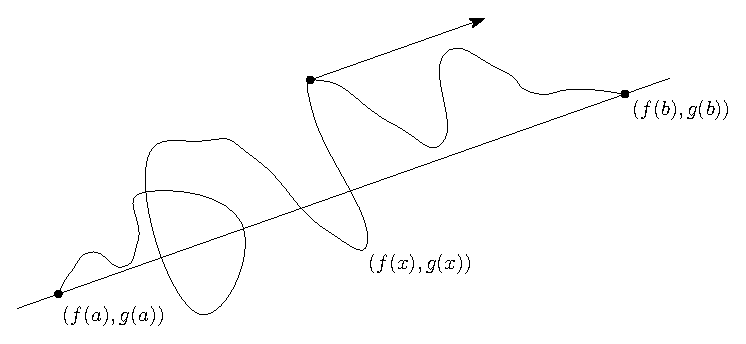
\includegraphics[width=0.55\textwidth]{24_1.eps}
	\caption{Геометрический смысл теоремы Коши.}
	\label{24_1}
\end{figure}
Вектор $(f(b) - f(a), g(b) - g(a))$ соединяет начало и конец маршрута, то есть это перемещение (насколько мы переместились), $(f^\prime(c),g^\prime(c))$ это вектор скорости. Таким образом был момент, когда вектор скорости коллинеарен вектору перемещения.

\begin{proof}
	Рассмотрим функцию 
	$F(x) = 
	\begin{vmatrix}
		f(b) - f(a) & f(x)\\
		g(b) - g(a) & g(x)
	\end{vmatrix} = (f(b) - f(a)){\cdot}g(x) - (g(b) - g(a)){\cdot}f(x)$. По свойству определителя 
	$F(a) = 
	\begin{vmatrix}
		f(b) - f(a) & f(a)\\
		g(b) - g(a) & g(a)
	\end{vmatrix} =
	\begin{vmatrix}
		f(b) & f(a) \\
		g(b) & g(a) 
	\end{vmatrix}$, 
	$F(b) = 
	\begin{vmatrix}
		-f(a) & f(b) \\
		-g(a) & g(b) 
	\end{vmatrix} = 
	\begin{vmatrix}
		f(b) & f(a) \\
		g(b) & g(a) 
	\end{vmatrix} 
	= F(a) \Rightarrow$ по теореме Ролля $\exists \, c \in(a,b) \colon F^\prime(c) = 0 \Rightarrow$ 
	$$F^\prime(c) = (f(b) - f(a)){\cdot}g^\prime(c) - (g(b) - g(a)){\cdot}f^\prime(c) = 0 \Rightarrow (f(b) - f(a)){\cdot}g^\prime(c) = (g(b) - g(a)){\cdot}f^\prime(c)$$
\end{proof}
\newpage
\section*{Правило Лопиталя}

\begin{theorem}\textbf{(Бернулли-Лопиталь)}
	Пусть $f$ и $g$ дифференцируемы на интервале $(a,b)$ и $g^\prime \neq 0$. Предположим, что выполняется одно из следующих двух условий:
	\begin{enumerate}[label={(\Roman*)}]
		\item $\!\lim\limits_{x \to b-}f(x) = \! \lim\limits_{x \to b-}g(x) = 0$;
		\item $\lim\limits_{x \to b-}g(x) = \infty$;
	\end{enumerate}
	Тогда, если $\lim\limits_{x \to b-}\dfrac{f^\prime(x)}{g^\prime(x)} = A$, то существует предел $\lim\limits_{x \to b-}\dfrac{f(x)}{g^(x)} = A$.
\end{theorem}
\subsection*{Условие $(\RN{2})$}
\uline{\textbf{Идея}}: В этом случае $\lim\limits_{x \to b-}g(x) = \infty$. Возьмем интервал $(a,b)$, возьмем на нём точки $y, x \colon x > y$. 
Применим к ним теорему Коши: 
$$\dfrac{f(x) - f(y)}{g(x) - g(y)} = \dfrac{f^\prime(c)}{g^\prime(c)} \Rightarrow \dfrac{f(x)}{g(x)} = \dfrac{f^\prime(c)}{g^\prime(c)} \bigg(1 - \dfrac{g(y)}{g(x)} \bigg) + \dfrac{f(y)}{g(x)}$$
Мы знаем, что $\lim\limits_{x \to b-}g(x) = \infty \wedge \lim\limits_{x \to b-}\dfrac{f^\prime(x)}{g^\prime(x)} = A \Rightarrow$ возьмем $y$ столь близко к $b$, что $\dfrac{f^\prime}{g^\prime} \approx A$, зафиксируем его. 
\begin{figure}[H]
	\centering
	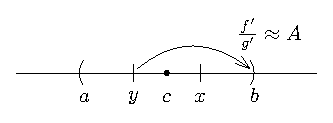
\includegraphics[width=0.35\textwidth]{24_2.eps}
	\caption{Идея доказательства теоремы Бернули-Лопиталя.}
	\label{24_2}
\end{figure}
Будем двигать $x$ к $b \Rightarrow$ будет изменяться $c$, но $c$ как бы не менялось будет лежать еще ближе к $b \Rightarrow$ в точке $c$ выражение $\dfrac{f^\prime}{g^\prime} \approx A$. Двигая $x$ к $b$ получим: $\bigg(1 - \dfrac{g(y)}{g(x)} \bigg) \approx 1, \, \dfrac{f(y)}{g(x)} \approx 0 \Rightarrow \dfrac{f(x)}{g(x)} \approx  \dfrac{f^\prime(c)}{g^\prime(c)} \approx A$. 
\begin{proof} 
	Пусть $\VE > 0, \exists \, y \colon  \forall z \in (y,b), \, \bigg|\dfrac{f^\prime(z)}{g^\prime(z)} - A\bigg| < \VE, \, \bigg|\dfrac{f^\prime(z)}{g^\prime(z)}\bigg| < C$, поскольку если предел есть, то функция ограничена в некоторой окрестности предельной точки. 
	
	Фиксируем $y$, $\exists \, \delta >0 \colon y < b -\delta \wedge \forall x \in (b -\delta,b), \, \bigg| \dfrac{g(y)}{g(x)} \bigg|< \VE \wedge \bigg|\dfrac{f(y)}{g(x)}\bigg| < \VE$, поскольку $f(y),g(y)$ - константы и $\!\lim\limits_{x \to b-}g(x) = \infty$. Таким образом, применяя теорему Коши и неравенство треугольника получим
	$$\forall x \in (b-\delta, b), \, \bigg|\dfrac{f(x)}{g(x)} - A \bigg| = \bigg|\dfrac{f^\prime(c)}{g^\prime(c)}  - \dfrac{f^\prime(c)}{g^\prime(c)}{\cdot}\dfrac{g(y)}{g(x)} + \dfrac{f(y)}{g(x)} - A \bigg| \leq \bigg|\dfrac{f^\prime(c)}{g^\prime(c)} - A \bigg| + \bigg|\dfrac{f^\prime(c)}{g^\prime(c)} \bigg|{\cdot}\bigg|\dfrac{g(y)}{g(x)}\bigg| + \bigg|\dfrac{f(y)}{g(x)}\bigg| \Rightarrow $$
	$$\Rightarrow \bigg|\dfrac{f(x)}{g(x)} - A \bigg| < \VE + C{\cdot}\bigg|\dfrac{g(y)}{g(x)}\bigg| + \bigg|\dfrac{f(y)}{g(x)}\bigg| < \VE + C{\cdot}\VE + \VE = (C+ 2)\VE$$
\end{proof}

\begin{rem}
	Точка $b$ не обязательно должна быть конечной и в этом случае, доказательство будет аналогичным.
\end{rem}

\subsection*{Условие $(\RN{1})$}
\uline{\textbf{Идея}}: В этом случае $\!\lim\limits_{x \to b-}f(x) = \! \lim\limits_{x \to b-}g(x) = 0$. Возьмем интервал $(a,b)$, возьмем на нём точки $x, y \colon x < y$. 
Применим к ним теорему Коши: 
$$\dfrac{f(y) - f(x)}{g(y) - g(x)} = \dfrac{f^\prime(c)}{g^\prime(c)} \Rightarrow \dfrac{f(x)}{g(x)} = \dfrac{f^\prime(c)}{g^\prime(c)} \bigg(1 - \dfrac{g(y)}{g(x)} \bigg) + \dfrac{f(y)}{g(x)}$$
Есть окрестность точки $b, \, (b-\delta,b)$ в которой $\dfrac{f^\prime}{g^\prime} \approx A$, зафиксируем в этой окрестности точку $x$, а точку $y$ будем менять. Тогда, точка $c$ будет лежать в этой же окрестности $\Rightarrow \dfrac{f^\prime}{g^\prime} \approx A \wedge x$ - зафиксирована $\Rightarrow$\\ 
$\Rightarrow g(x) = \text{const} \wedge  \!\lim\limits_{y \to b-}g(y) = \!\lim\limits_{y \to b-}f(y) = 0 \Rightarrow \bigg(1 - \dfrac{g(y)}{g(x)} \bigg) \to 1, \, \dfrac{f(y)}{g(x)} \to 0 \Rightarrow \dfrac{f(x)}{g(x)} \approx  \dfrac{f^\prime(c)}{g^\prime(c)} \approx A$ в окрестности $b$.
\begin{proof}
	Пусть $\VE > 0, \exists \, x \colon  \forall z \in (x,b), \, \bigg|\dfrac{f^\prime(z)}{g^\prime(z)} - A\bigg| < \VE, \, \bigg|\dfrac{f^\prime(z)}{g^\prime(z)}\bigg| < C$, поскольку если предел есть, то функция ограничена в некоторой окрестности предельной точки. 
	
	Фиксируем $x$, $\exists \, \delta >0 \colon x < b -\delta \wedge \forall y \in (b -\delta,b), \, \bigg| \dfrac{g(y)}{g(x)} \bigg|< \VE \wedge \bigg|\dfrac{f(y)}{g(x)}\bigg| < \VE$, поскольку $f(x),g(x)$ - константы и $\!\lim\limits_{y \to b-}g(y) = \!\lim\limits_{y \to b-}f(y) = 0$. Таким образом, применяя теорему Коши и неравенство треугольника получим
	$$\forall y \in (b-\delta, b), \, \bigg|\dfrac{f(x)}{g(x)} - A \bigg| = \bigg|\dfrac{f^\prime(c)}{g^\prime(c)}  - \dfrac{f^\prime(c)}{g^\prime(c)}{\cdot}\dfrac{g(y)}{g(x)} + \dfrac{f(y)}{g(x)} - A \bigg| \leq \bigg|\dfrac{f^\prime(c)}{g^\prime(c)} - A \bigg| + \bigg|\dfrac{f^\prime(c)}{g^\prime(c)} \bigg|{\cdot}\bigg|\dfrac{g(y)}{g(x)}\bigg| + \bigg|\dfrac{f(y)}{g(x)}\bigg| \Rightarrow $$
	$$\Rightarrow \bigg|\dfrac{f(x)}{g(x)} - A \bigg| < \VE + C{\cdot}\bigg|\dfrac{g(y)}{g(x)}\bigg| + \bigg|\dfrac{f(y)}{g(x)}\bigg| < \VE + C{\cdot}\VE + \VE = (C+ 2)\VE$$
\end{proof}

\begin{proof} \textbf{Случай $A = +\infty$}:\\
	Пусть $M > 0, \exists \, x \colon  \forall z \in (x,b), \, \dfrac{f^\prime(z)}{g^\prime(z)} > M$. То есть для любого наперед фиксированного числа, найдется большее значение функции $\dfrac{f^\prime}{g^\prime}$.
	
	Фиксируем $x$, пусть $M > \VE > 0, \exists \, \delta >0 \colon x < b -\delta \wedge \forall y \in (b -\delta,b), \, \bigg| \dfrac{g(y)}{g(x)} \bigg|< \VE \wedge \bigg|\dfrac{f(y)}{g(x)}\bigg| < \VE$, поскольку $f(x),g(x)$ - константы и $\!\lim\limits_{y \to b-}g(y) = \!\lim\limits_{y \to b-}f(y) = 0$. Таким образом, применяя теорему Коши получим
	$$\forall y \in (b-\delta, b), \, \dfrac{f(x)}{g(x)} = \dfrac{f^\prime(c)}{g^\prime(c)}\bigg(1  - \dfrac{g(y)}{g(x)}\bigg) + \dfrac{f(y)}{g(x)}  > M(1 + \VE) - \VE > M -\VE = \tilde{M} >0$$ 	
\end{proof}

\newpage
\section*{Многочлен Тейлора}
\subsection*{Многочлен $\Rightarrow$ коэффициенты}

Возьмем многочлен $P(x) = c_0 + c_1(x-a) + c_2(x-a)^2 + \dotsc + c_n(x-a)^n$ (разложение многочлена $P$ в точке $a$ по степеням $(x-a)$). Как найти коэффициенты такого разложения? 

\begin{enumerate}
	\item [$c_0$:] Ясно, что $c_0 = P(a)$;
	\item [$c_1$:] Продифференцируем многочлен $\Rightarrow P^\prime(x) = c_1 + 2c_2(x-a) + \dotsc + nc_n(x-a)^{n-1} \Rightarrow  c_1 = P^\prime(a)$;
	\item [$c_2$:] Продифференцируем $P^{\prime}(x) \Rightarrow P^{\prime\prime}(x) = 2c_2 + 3{\cdot}2c_3(x-a) + \dotsc \Rightarrow c_2 = \dfrac{P^{\prime\prime}(a)}{2}$;
\end{enumerate}

Продолжая эти рассуждения мы получаем, что $k$-ый коэффициент
$$c_k = \dfrac{P^{(k)}(a)}{k!}$$
Теперь вместо коэффициентов в $P(x)$ мы можем написать их выражение через производные в точке и получим следующий вид многочлена:
$$P(x) = P(a) + P^\prime(a)(x-a) + \dotsc + \dfrac{P^{(n)}(a)}{n!}(x-a)^n$$
\begin{rem}
	Отметим, что такое производная $k$-го порядка: Если мы уже знаем, что такое производная $k$-го порядка и эта производная есть в окрестности точки $a$, тем самым в окрестности точки $a$ определена функция $f^{(k)}(x)$ и если она оказалась дифференцируемой в точке $a$, то её производная в точке $a$ и будет производной следующего порядка: $(f^{(k)}(a))^\prime = f^{(k+1)}(a)$.
\end{rem}

\textbf{Пример}: $f(x) = x^m \Rightarrow f^{(k)}(x) = (x^m)^{(k)} = 
\begin{cases}
	0 & k > m \\
	m! & k = m\\
	m(m-1){\cdot}\dotsc{\cdot}(m-k+1)x^{m-k} & k < m
\end{cases}
$

\begin{exrc}\textbf{Обобщенное правило Лейбница}:
	Доказать $(fg)^{(n)} = \displaystyle\sum\limits_{k=0}^{n}C_n^kf^{(k)}{\cdot}g^{(n-k)}$.
\end{exrc}
\begin{proof}
	Докажем по индукции:\\
	\uline{\textbf{База}}: обычное правило Лейбница $(fg)^\prime = f^\prime g + fg^\prime$.
	
	\uline{\textbf{Шаг}}: пусть доказано для $n$, докажем для $n +1$:
	$$(fg)^{(n+1)} = \sum\limits_{k=0}^{n}C_n^kf^{(k)}g^{(n + 1 - k)} + \sum\limits_{k=0}^{n}C_n^kf^{(k + 1)}g^{(n - k)} = C_n^0fg^{(n+1)} + \sum\limits_{k=1}^{n}C_n^kf^{(k)}g^{(n + 1 - k)} + \sum\limits_{k=1}^{n+1}C_n^{k-1}f^{(k)}g^{(n + 1 - k)} =
	$$
	$$= fg^{(n+1)} + \sum\limits_{k=1}^{n}C_n^kf^{(k)}g^{(n + 1 - k)} + \sum\limits_{k=1}^{n}C_n^{k-1}f^{(k)}g^{(n + 1 - k)} + C_n^n f^{(n+1)}g = fg^{(n+1)} + \sum\limits_{k=1}^{n} \Big( C_n^k + C_n^{k-1} \Big)f^{(k)}g^{(n + 1 - k)} + 
	$$
	$$
	 + f^{(n+1)}g = fg^{(n+1)} + \sum\limits_{k=1}^{n} C_{n+1}^k f^{(k)}g^{(n + 1 - k)} + f^{(n+1)}g = \sum\limits_{k=0}^{n + 1} C_{n+1}^k f^{(k)}g^{(n + 1 - k)}
	$$
\end{proof}

\subsection*{Коэффициенты $\Rightarrow$ многочлен}

Теперь посмотрим на обратную задачу: выписать многочлен, если заданы производные в точке $a$. Если нужен многочлен с заданными первыми $n$ производными, то он будет следующего вида:
$$P(x) = P(a) + P^\prime(a)(x-a) + \dotsc + \dfrac{P^{(n)}(a)}{n!}(x-a)^n$$

Пусть $f$ это $n$-раз дифференцируемая функция в точке $a$. 
\begin{defn}
	Многочлен у которого производные такие же, как у функции $f$ называется \uwave{многочленом Тейлора}:
	$$\MT_n(x) =\sum\limits_{k = 0}^{n}\dfrac{f^{(k)}(a)}{k!}(x-a)^k, \, f^{(k)}(a) = \big(\MT_n(x) \big)^{(k)}\Big|_{x = a}, \, \forall k = \overline{0,n}$$
\end{defn}

Рассмотрим функцию $$g(x) = f(x) - \MT_n(x), \, g^{(k)}(a) = 0, \, \forall k = \overline{0,n}$$ 
У какой функции все производные до $n$-го порядка в точке $a$ равны нулю? Например, у $(x-a)^{n+1}$.

\begin{theorem}
	Если $f$ $n$-раз дифференцируема в точке $a$, то $f(x) - T_n(x) = \alpha(x){\cdot}(x-a)^n$, где $\lim\limits_{x \to a} \alpha(x) = 0$
\end{theorem}

Это утверждение можно записать короче, использяу $\bar{o}$-символику:
$$h(x) = \alpha(x){\cdot}g(x), \, x\neq a \wedge \lim\limits_{x\to a} \alpha(x) = 0 \Rightarrow h = \bar{o}(g) \text{, при $x \to a$ }$$
Тогда теорему перепишем в виде \uline{\textbf{формулы Тейлора с остаточным членом в форме Пеано}}:
$$f(x) = T_n(x) +  \bar{o}((x-a)^n) \text{, при $x \to a$ }$$

\end{document}